\chapter{Bidirectional Long Short Term Memory Network Models}
In this chapter, we first describe the Bidirectional Long Short Term Memory network (BiLSTM) and Character Embeddings. Then, we show the performance and decoding speed of the sequence tagging systems with different BiLSTM configurations.

\section{Model Description}
\subsection{Bidirectional Bidirectional Long Short Term Memory}

One major disadvantage of feedforward neural networks is that they only consider the context of the focus word instead of the whole sequence. Recurrent neural networks (RNNs) (\citeauthor{mikolov2010recurrent}, \citeyear{mikolov2010recurrent}) can keep the future and the past data to persist by using memory cells with loops in them. However, RNNs is biased towards the most recent data in practice. Long Short Term Memory Networks (LSTMs), special RNNs with Long Short Term memory cells  (\citeauthor{graves2005framewise}, \citeyear{graves2005framewise}), are designed to combat the bias problem. LSTMs learn long dependencies in a sequence with help of the structure of Gates (\citeauthor{graves2005framewise}, \citeyear{graves2005framewise}). Gates control how much of the input is given to the next LSTM cell, and how much of the previous information to forget.

Given a sentence with $n$ words each of which is represented as a dense vector $x_i$, a LSTM makes use of $x_{1:n}$ to compute a forward representation $\overrightarrow {h_{i}}$ for the $i$th word. In general, computing a backward representation $\overleftarrow {h_{i}}$ would be useful for sequence tagging. Bidirectional LSTM (BiLSTM) is an extension to LSTM which take into account both the past data and the future data in a sequence. A BiLSTM generates both $\overrightarrow {h_{i}}$ and $\overleftarrow {h_{i}}$ for the $i$th word in the sequence. The hidden embedding $h_{i}$ is the concatenation of $\overrightarrow {h_{i}}$ and $\overleftarrow {h_{i}}$. The BiLSTM mapping is defined as $BiLSTM_{\theta}$:
$h_{i} = BiLSTM_{\theta}\left(x_{1:n}, i\right)$ where $\theta$ represents trainable parameters in BiLSTM.

 We can combine BiLSTM with CRF to make use of sentence level tag information. As in the Feedforward-CRF model, we introduce a transition matrix $T$ to keep the transition score from $y_{i}$ to $y_{i+1}$. Given an output sequence $Y$, the score of the output sequence is given by:

\begin{equation}
S\left( X|Y\right)=\sum _{i}^{n}T_{i,i+1}+\sum _{i}^{n}P_{i}
\end{equation}

We can use dynamic program to compute the transition matrix and find the optimal output tag sequence. Figure \ref{fig:bilstmcrf} illustrates the BiLSTM model with CRF on a NER example.

\begin{figure}
  \centering
  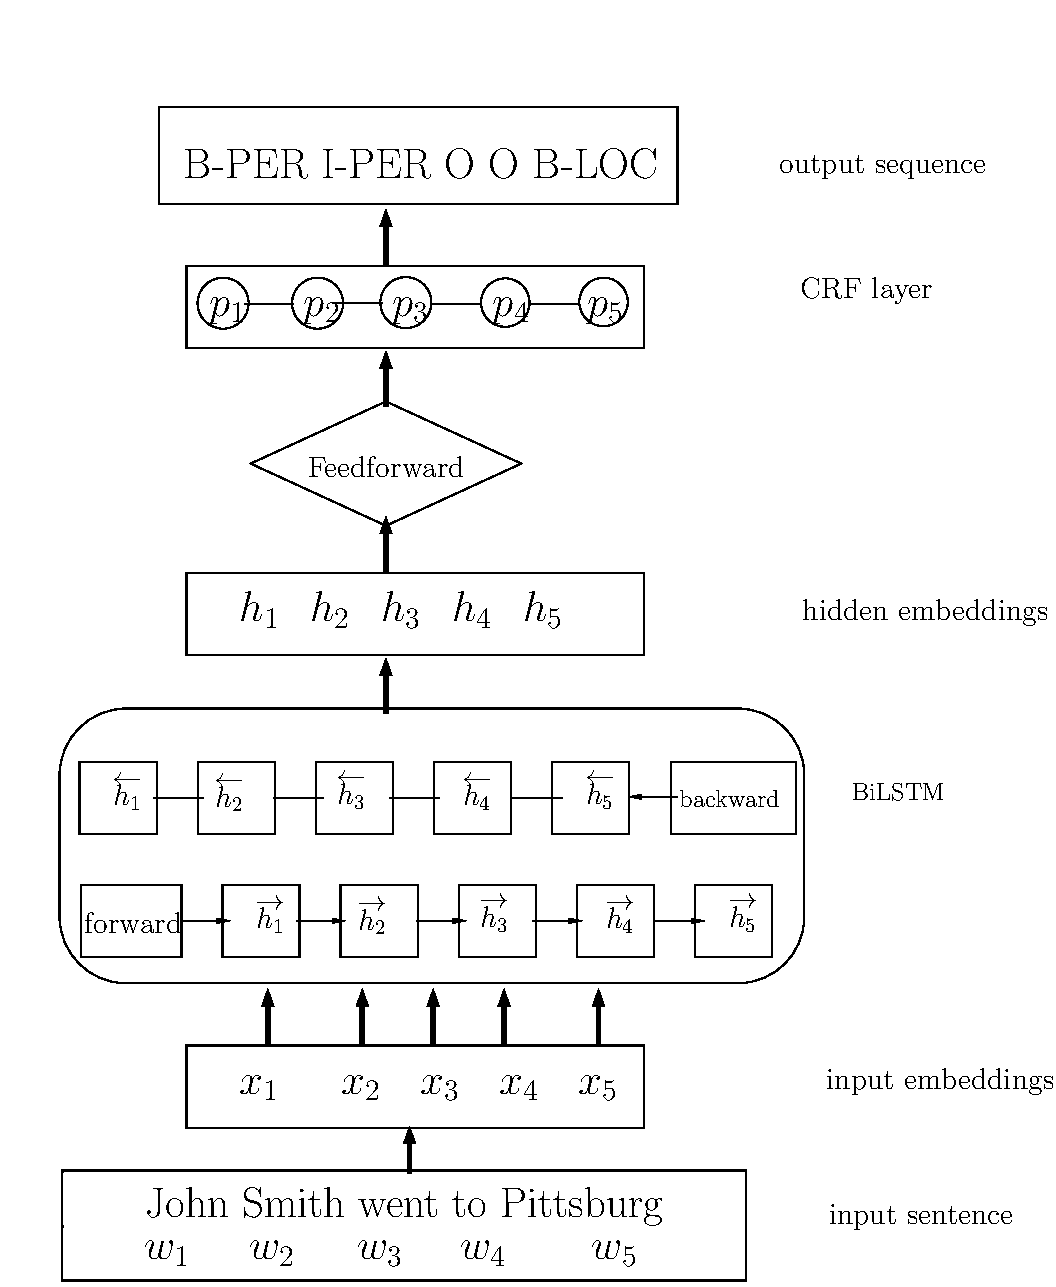
\includegraphics[scale=0.6]{bilstmcrf.pdf}
 \caption{The architecture of the tagging system using BiLSTM with CRF}
  \label{fig:bilstmcrf}
\end{figure}

\subsection{Character Embeddings}

Instead of using hand-engineered features listed in Chapter 2 (like the prefixes and the suffixes of a word), we can use a BiLSTM network to construct word representations from the characters in it (\citeauthor{lample2016neural}, \citeyear{lample2016neural}). This architecture is denoted as Character Embeddings. It's been shown that learning character embeddings has been found useful for capturing morphological evidence (\citeauthor{ling2015finding}, \citeyear{ling2015finding}). Figure \ref{fig:charlstm} describes the architecture of the using Character Embeddings and BiLSTM to generate word embeddings. The input to the BiLSTM in Character Embeddings is the letter sequence of a word. We define a character dictionary which maps each character to a $d$-dimensional vector representation. The English character dictionary contains uppercase and lowercase letters, numbers, and punctuation. We look up each $c_{i}$ of the input letter sequence from the dictionary and get the input character vectors $X:\left\{x_{1},x_{2},\dots,x_{n}\right\}$. Then, the input character vectors $X$ is fed into BiLSTM to generate forward and backward hidden embeddings of the character sequence. We concatenate the last forward hidden embedding $\overrightarrow {h_{n}}$ and the last backward hidden embedding $\overrightarrow {h_{1}}$ with the embedding from the word vector dictionary to obtain the final word embedding.

We add Character Embeddings into the tagging system by concatenating the output of Character Embeddings and the word embeddings from lookup to form the input embeddings. Then, we feed the input embeddings to BiLSTM and CRF, and we get the fully structured BiLSTM model (BiLSTM-Char-CRF) for sequence tagging. The character embeddings and word embeddings are learned together during training. There are existing implementations of this BiLSTM-Char-CRF model, such as NeuroNet by \cite{2017neuroner}. We re-implement BiLSTM-Char-CRF for the comparison with other models in this thesis.

\begin{figure}
  \centering
  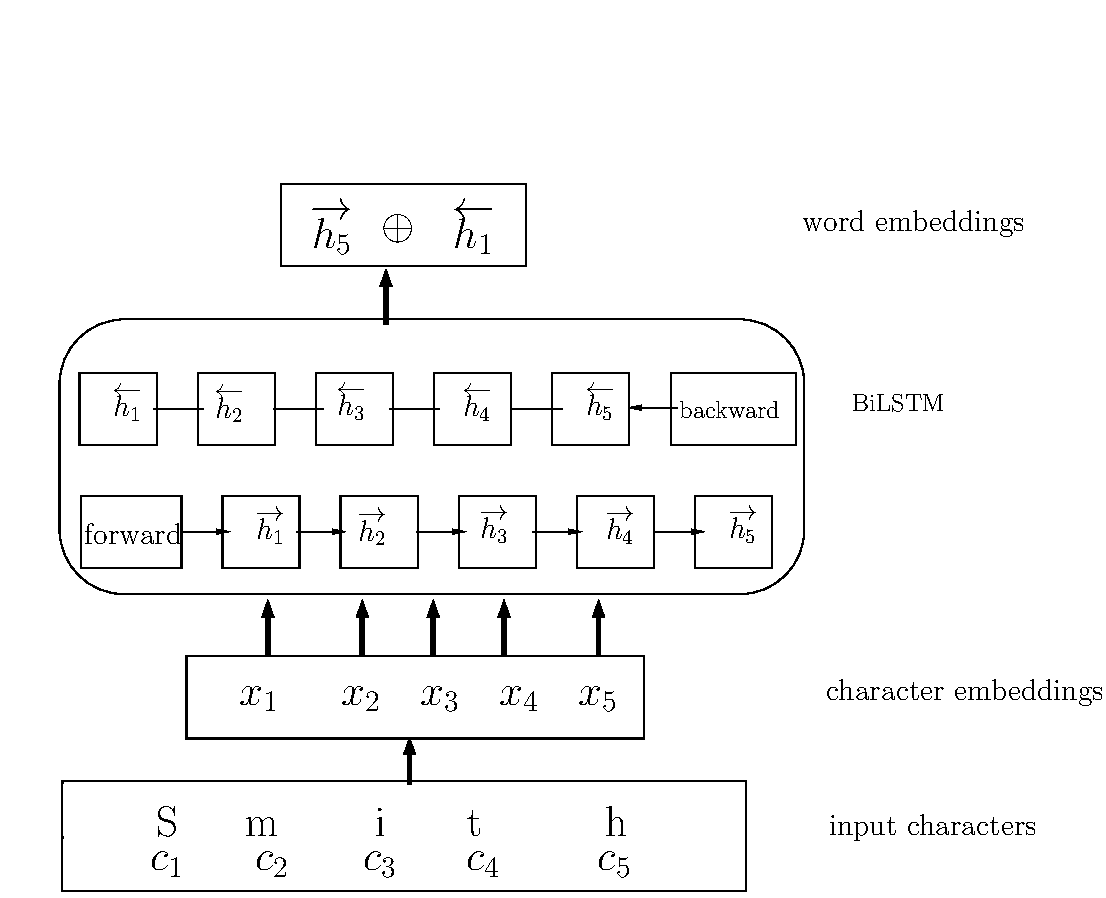
\includegraphics[scale=0.6]{bilstmchar.pdf}
 \caption{The word embedding derived from the character embeddings}
  \label{fig:charlstm}
\end{figure}


 
\section{Experiments and Results}

To evaluate BiLSTM models, we run BiLSTM with three configurations on POS and NER: BiLSTM with word features only (BiLSTM); BiLSTM with Character Embeddings (BiLSTM-Char); BiLSTM with Character Embeddings and a CRF layer (BiLSTM-Char-CRF). We report the performance and decoding speed of the models on Penn Treebank data set for POS, and on CoNLL 2003 data set for NER. 

We implement the BiLSTM models using Python and the Tensorflow 1.0 library. The hidden layer size in the BiLSTM of Character Embeddings is set to 25, and the hidden layer size in word sequence BiLSTM is set to 100. The rest of the hyperparameters are the same as the ones in the experiments in Chapter 2. Since dropout training (\citeauthor{hinton2012improving}, \citeyear{hinton2012improving}) can improve the performance by encouraging the model to depend on both character embeddings and word embeddings, we apply a dropout mask on the input embeddings before the BiLSTM layer. The dropout rate is set to 0.5 in the experiments. Table \ref{table:hyperparameters2} shows the hyperparameters used in BiLSTM models.

\begin{table}[]
\centering
\caption{Hyperparameters used in BiLSTM Models}
\label{table:hyperparameters2}
\begin{tabular}{|c|c|}
\hline
Hyperparameters & Values \\ \hline
character embedding size & 50 \\ \hine
word embedding size & 100 \\ \hline
feedforward layer size & 200 \\ \hline
LSTM layer size & 200 \\ \hline
optimizer & Adam \\ \hline
learning rate & 0.01 \\ \hline
batch size & 32 \\ \hline
\end{tabular}
\end{table}

Figure \ref{fig:lstmbar} illustrates the performance of BiLSTM, BiLSTM-Char, BiLSTM-Char-CRF. As expected, the fully structured BiLSTM model outperforms the other two. Character Embedding increases the POS accuracy by 1.17, and increases the NER F1 score by 3.34. It reveals that the BiLSTM networks do not heavily depend on features other than words, and Character Embeddings can help improve the performance of the models. Compared to BiLSTM-Char, BiLSTM-Char-CRF improves the POS performance by 0.13, and improves the NER performance by 1.79. CRF layer is more helpful for NER for the reason that there are grammar constrains on NER tags.

Table \ref{table:lstm-table1} and Table \ref{table:lstm-table2} describe the final results of the performance and decoding speed of the BiLSTM models on the POS and NER. It is obvious that the more features the model has, the slower it would be. Adding a CRF layer will increase the performance but decrease the decoding time. Table \ref{table:lstm-table3} benchmarks the fully structured BiLSTM-Char-CRF model against Feedforward-History and Feedforward-CRF.

\begin{figure}
  \centering
  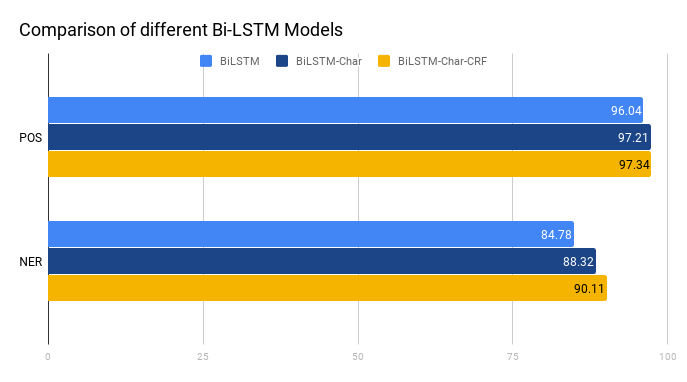
\includegraphics[scale=0.6]{lstmbar.png}
 \caption{Performance comparison between BiLSTM models on POS and NER}
  \label{fig:lstmbar}
\end{figure}

\begin{table}[]
\centering
\caption{BiLSTM Models Accuracy and F1 Score}
\label{table:lstm-table1}
\begin{tabular}{|c|c|c|}
\hline
Model         & POS (Accuracy)  & NER (F-Score)       \\ \hline
BiLSTM  & 96.01     & 84.78                             \\ \hline
BiLSTM-Char & 97.21 & 88.32             \\ \hline
BiLSTM-Char-CRF & \textbf{97.34}  & \textbf{90.11}             \\ \hline
\end{tabular}
\end{table}

\begin{table}[]
\centering
\caption{BiLSTM Models Decoding Speed}
\label{table:lstm-table2}
\begin{tabular}{|c|c|c|}
\hline
Model       & POS  (sentences, words/sec)  & NER  (sentences, words/sec)      \\ \hline
BiLSTM             & 981(23036)     & 1637(20740)       \\ \hline
BiLSTM-Char        & 596(13992)  & 889(11271)             \\ \hline
BiLSTM-Char-CRF    & 383(9009)  & 795(10100)         \\ \hline
\end{tabular}
\end{table}

\begin{table}[]
\centering
\caption{Decoding Speed Comparison between BiLSTM Models and Feedforward Models on POS and NER}
\label{table:lstm-table3}
\begin{tabular}{|c|c|c|}
\hline
Model       & POS  (sentences, words/sec)  & NER  (sentences, words/sec)      \\ \hline
Feedforward-History            & 829(19474)     & 1390(17609)       \\ \hline
Feedforward-CRF        & 761(17877)  & 1374(17412)             \\ \hline
BiLSTM-Char-CRF    & 383(9009)  & 795(10100)         \\ \hline
\end{tabular}
\end{table}

